% Options for packages loaded elsewhere
\PassOptionsToPackage{unicode}{hyperref}
\PassOptionsToPackage{hyphens}{url}
%
\documentclass[
]{book}
\title{ImpactTB/BAA: Standard Operating Procedures for Data Analysis}
\author{Colorado State University Coding Team}
\date{2022-07-07}

\usepackage{amsmath,amssymb}
\usepackage{lmodern}
\usepackage{iftex}
\ifPDFTeX
  \usepackage[T1]{fontenc}
  \usepackage[utf8]{inputenc}
  \usepackage{textcomp} % provide euro and other symbols
\else % if luatex or xetex
  \usepackage{unicode-math}
  \defaultfontfeatures{Scale=MatchLowercase}
  \defaultfontfeatures[\rmfamily]{Ligatures=TeX,Scale=1}
\fi
% Use upquote if available, for straight quotes in verbatim environments
\IfFileExists{upquote.sty}{\usepackage{upquote}}{}
\IfFileExists{microtype.sty}{% use microtype if available
  \usepackage[]{microtype}
  \UseMicrotypeSet[protrusion]{basicmath} % disable protrusion for tt fonts
}{}
\makeatletter
\@ifundefined{KOMAClassName}{% if non-KOMA class
  \IfFileExists{parskip.sty}{%
    \usepackage{parskip}
  }{% else
    \setlength{\parindent}{0pt}
    \setlength{\parskip}{6pt plus 2pt minus 1pt}}
}{% if KOMA class
  \KOMAoptions{parskip=half}}
\makeatother
\usepackage{xcolor}
\IfFileExists{xurl.sty}{\usepackage{xurl}}{} % add URL line breaks if available
\IfFileExists{bookmark.sty}{\usepackage{bookmark}}{\usepackage{hyperref}}
\hypersetup{
  pdftitle={ImpactTB/BAA: Standard Operating Procedures for Data Analysis},
  pdfauthor={Colorado State University Coding Team},
  hidelinks,
  pdfcreator={LaTeX via pandoc}}
\urlstyle{same} % disable monospaced font for URLs
\usepackage{color}
\usepackage{fancyvrb}
\newcommand{\VerbBar}{|}
\newcommand{\VERB}{\Verb[commandchars=\\\{\}]}
\DefineVerbatimEnvironment{Highlighting}{Verbatim}{commandchars=\\\{\}}
% Add ',fontsize=\small' for more characters per line
\usepackage{framed}
\definecolor{shadecolor}{RGB}{248,248,248}
\newenvironment{Shaded}{\begin{snugshade}}{\end{snugshade}}
\newcommand{\AlertTok}[1]{\textcolor[rgb]{0.94,0.16,0.16}{#1}}
\newcommand{\AnnotationTok}[1]{\textcolor[rgb]{0.56,0.35,0.01}{\textbf{\textit{#1}}}}
\newcommand{\AttributeTok}[1]{\textcolor[rgb]{0.77,0.63,0.00}{#1}}
\newcommand{\BaseNTok}[1]{\textcolor[rgb]{0.00,0.00,0.81}{#1}}
\newcommand{\BuiltInTok}[1]{#1}
\newcommand{\CharTok}[1]{\textcolor[rgb]{0.31,0.60,0.02}{#1}}
\newcommand{\CommentTok}[1]{\textcolor[rgb]{0.56,0.35,0.01}{\textit{#1}}}
\newcommand{\CommentVarTok}[1]{\textcolor[rgb]{0.56,0.35,0.01}{\textbf{\textit{#1}}}}
\newcommand{\ConstantTok}[1]{\textcolor[rgb]{0.00,0.00,0.00}{#1}}
\newcommand{\ControlFlowTok}[1]{\textcolor[rgb]{0.13,0.29,0.53}{\textbf{#1}}}
\newcommand{\DataTypeTok}[1]{\textcolor[rgb]{0.13,0.29,0.53}{#1}}
\newcommand{\DecValTok}[1]{\textcolor[rgb]{0.00,0.00,0.81}{#1}}
\newcommand{\DocumentationTok}[1]{\textcolor[rgb]{0.56,0.35,0.01}{\textbf{\textit{#1}}}}
\newcommand{\ErrorTok}[1]{\textcolor[rgb]{0.64,0.00,0.00}{\textbf{#1}}}
\newcommand{\ExtensionTok}[1]{#1}
\newcommand{\FloatTok}[1]{\textcolor[rgb]{0.00,0.00,0.81}{#1}}
\newcommand{\FunctionTok}[1]{\textcolor[rgb]{0.00,0.00,0.00}{#1}}
\newcommand{\ImportTok}[1]{#1}
\newcommand{\InformationTok}[1]{\textcolor[rgb]{0.56,0.35,0.01}{\textbf{\textit{#1}}}}
\newcommand{\KeywordTok}[1]{\textcolor[rgb]{0.13,0.29,0.53}{\textbf{#1}}}
\newcommand{\NormalTok}[1]{#1}
\newcommand{\OperatorTok}[1]{\textcolor[rgb]{0.81,0.36,0.00}{\textbf{#1}}}
\newcommand{\OtherTok}[1]{\textcolor[rgb]{0.56,0.35,0.01}{#1}}
\newcommand{\PreprocessorTok}[1]{\textcolor[rgb]{0.56,0.35,0.01}{\textit{#1}}}
\newcommand{\RegionMarkerTok}[1]{#1}
\newcommand{\SpecialCharTok}[1]{\textcolor[rgb]{0.00,0.00,0.00}{#1}}
\newcommand{\SpecialStringTok}[1]{\textcolor[rgb]{0.31,0.60,0.02}{#1}}
\newcommand{\StringTok}[1]{\textcolor[rgb]{0.31,0.60,0.02}{#1}}
\newcommand{\VariableTok}[1]{\textcolor[rgb]{0.00,0.00,0.00}{#1}}
\newcommand{\VerbatimStringTok}[1]{\textcolor[rgb]{0.31,0.60,0.02}{#1}}
\newcommand{\WarningTok}[1]{\textcolor[rgb]{0.56,0.35,0.01}{\textbf{\textit{#1}}}}
\usepackage{longtable,booktabs,array}
\usepackage{calc} % for calculating minipage widths
% Correct order of tables after \paragraph or \subparagraph
\usepackage{etoolbox}
\makeatletter
\patchcmd\longtable{\par}{\if@noskipsec\mbox{}\fi\par}{}{}
\makeatother
% Allow footnotes in longtable head/foot
\IfFileExists{footnotehyper.sty}{\usepackage{footnotehyper}}{\usepackage{footnote}}
\makesavenoteenv{longtable}
\usepackage{graphicx}
\makeatletter
\def\maxwidth{\ifdim\Gin@nat@width>\linewidth\linewidth\else\Gin@nat@width\fi}
\def\maxheight{\ifdim\Gin@nat@height>\textheight\textheight\else\Gin@nat@height\fi}
\makeatother
% Scale images if necessary, so that they will not overflow the page
% margins by default, and it is still possible to overwrite the defaults
% using explicit options in \includegraphics[width, height, ...]{}
\setkeys{Gin}{width=\maxwidth,height=\maxheight,keepaspectratio}
% Set default figure placement to htbp
\makeatletter
\def\fps@figure{htbp}
\makeatother
\setlength{\emergencystretch}{3em} % prevent overfull lines
\providecommand{\tightlist}{%
  \setlength{\itemsep}{0pt}\setlength{\parskip}{0pt}}
\setcounter{secnumdepth}{5}
\usepackage{booktabs}
\usepackage{amsthm}
\makeatletter
\def\thm@space@setup{%
  \thm@preskip=8pt plus 2pt minus 4pt
  \thm@postskip=\thm@preskip
}
\makeatother
\ifLuaTeX
  \usepackage{selnolig}  % disable illegal ligatures
\fi
\usepackage[]{natbib}
\bibliographystyle{apalike}

\begin{document}
\maketitle

{
\setcounter{tocdepth}{1}
\tableofcontents
}
\hypertarget{overview}{%
\chapter{Overview}\label{overview}}

Here, we have built a comprehensive guide to wet lab data collection, sample processing, and computational tool creation for robust and efficient data analysis and dissemination.

\hypertarget{introduction}{%
\chapter{Introduction}\label{introduction}}

\hypertarget{about-the-project-immune-mechanisms-of-protection-against-mycobacterium-tuberculosis-impac-tb}{%
\section{About the project: Immune Mechanisms of Protection against Mycobacterium tuberculosis (IMPAc-TB)}\label{about-the-project-immune-mechanisms-of-protection-against-mycobacterium-tuberculosis-impac-tb}}

The objective of the IMPAc-TB program is to get a thorough understanding of the immune responses necessary to avoid initial infection with \emph{Mycobacterium tuberculosis (Mtb)}, formation of latent infection, and progression to active TB illness. To achieve these goals, the National Institute of Allergy and Infectious Diseases awarded substantial funding and established multidisciplinary research teams that will analyze immune responses against \emph{Mtb} in animal models (mice, guinea pigs, and non-human primates) and humans, as well as immune responses elicited by promising vaccine candidates. The contract awards establish and give up to seven years of assistance for IMPAc-TB Centers to explain the immune responses required for \emph{Mtb} infection protection.

The seven centers that are part of the study are (in alphabetical order):

\begin{enumerate}
\def\labelenumi{\arabic{enumi}.}
\tightlist
\item
  Colorado State University
\item
  Harvard T.H. Chan School of Public Health
\item
  Seattle Children Hospital
\end{enumerate}

Colorado State University Team and role of each member:
Dr.~Marcela Henao-Tamayo: Principal Investigator
Dr.~Brendan Podell: Principal Investigator
Dr.~Andres Obregon-Henao: Research Scientist-III
Dr.~Taru S. Dutt: Research Scientist-I

\hypertarget{initial-mouse-characteristics}{%
\chapter{Initial mouse characteristics}\label{initial-mouse-characteristics}}

Here is a review of existing methods.

\hypertarget{mouse-weights}{%
\chapter{Mouse Weights}\label{mouse-weights}}

Mice are weighed in grams weekly to monitor clinical status as TB patients frequently display weight loss as clinical symptom associated with disease progression.

Weights are recorded in an excel worksheet.

Column titles are as follows: who\_collected date\_collected sex dob notch\_id mouse\_number weight unit cage\_number group notes

Groups included are: bcg, saline, bcg+id93, saline+id93, saline+noMtb

The notes column contains information regarding clinical observations.

good reference: \url{https://elifesciences.org/articles/74419\#s4}

\begin{Shaded}
\begin{Highlighting}[]
\FunctionTok{library}\NormalTok{(readxl)}
\FunctionTok{library}\NormalTok{(tidyverse)}
\end{Highlighting}
\end{Shaded}

\begin{verbatim}
## -- Attaching packages --------------------------------------- tidyverse 1.3.1 --
\end{verbatim}

\begin{verbatim}
## v ggplot2 3.3.5     v purrr   0.3.4
## v tibble  3.1.6     v dplyr   1.0.7
## v tidyr   1.1.4     v stringr 1.4.0
## v readr   2.1.1     v forcats 0.5.1
\end{verbatim}

\begin{verbatim}
## -- Conflicts ------------------------------------------ tidyverse_conflicts() --
## x dplyr::filter() masks stats::filter()
## x dplyr::lag()    masks stats::lag()
\end{verbatim}

\hypertarget{read-in-data}{%
\section{Read in data}\label{read-in-data}}

\hypertarget{data-is-stored-in-one-excel-sheet-each-week-is-one-sheet-named-as-the-date---return-vector-for-each-sheet-name}{%
\chapter{Data is stored in one excel sheet, each week is one sheet named as the date -\textgreater{} return vector for each sheet name}\label{data-is-stored-in-one-excel-sheet-each-week-is-one-sheet-named-as-the-date---return-vector-for-each-sheet-name}}

\hypertarget{can-also-use-rio-to-read-in-the-data-more-streamlined}{%
\chapter{can also use rio to read in the data, more streamlined}\label{can-also-use-rio-to-read-in-the-data-more-streamlined}}

\hypertarget{clean-data}{%
\section{Clean data}\label{clean-data}}

\begin{Shaded}
\begin{Highlighting}[]
\NormalTok{data}\SpecialCharTok{$}\NormalTok{before\_vaccination }\SpecialCharTok{\%\textgreater{}\%}
 \FunctionTok{select}\NormalTok{(}\StringTok{"sex"}\NormalTok{, }\StringTok{"notch\_id"}\NormalTok{,  }\StringTok{"weight"}\NormalTok{, }\StringTok{"cage\_number"}\NormalTok{, }\StringTok{"group"}\NormalTok{) }\CommentTok{\#"mouse\_number" it couldn\textquotesingle{}t find this for some reason }
\end{Highlighting}
\end{Shaded}

\begin{verbatim}
## [1] sex         notch_id    weight      cage_number group      
## <0 rows> (or 0-length row.names)
\end{verbatim}

\hypertarget{summary-statistics}{%
\section{Summary statistics}\label{summary-statistics}}

\hypertarget{body-weight-over-time-graph-and-statistics}{%
\chapter{Body weight over time graph and statistics}\label{body-weight-over-time-graph-and-statistics}}

\hypertarget{weight-loss-over-time-graph-and-statistics}{%
\chapter{Weight loss over time graph and statistics}\label{weight-loss-over-time-graph-and-statistics}}

\hypertarget{weight-vs-cfu}{%
\chapter{Weight vs CFU}\label{weight-vs-cfu}}

\hypertarget{weight-vs-elisa-results}{%
\chapter{Weight vs ELISA results}\label{weight-vs-elisa-results}}

\hypertarget{weight-vs-lesion-burden}{%
\chapter{Weight vs lesion burden}\label{weight-vs-lesion-burden}}

\hypertarget{colony-forming-units-to-determine-bacterial-counts}{%
\chapter{Colony forming units to determine bacterial counts}\label{colony-forming-units-to-determine-bacterial-counts}}

\hypertarget{data-description}{%
\section{Data description}\label{data-description}}

The data are collected in a spreadsheet with multiple sheets. The first sheet
(named ``{[}x{]}'') is used to record some metadata for the experiment, while the
following sheets are used to record CFUs counts from the plates used for samples
from each organ, with one sheet per organ. For example, if you plated data
from both the lung and spleen, there would be three sheets in the file: one
with the metadata, one with the plate counts for the lung, and one with the
plate counts for the spleen.

The metadata sheet is used to record information about the overall process of
plating the data. Values from this sheet will be used in calculating the bacterial
load in the original sample based on the CFU counts. This spreadsheet includes
the following columns:

\begin{itemize}
\tightlist
\item
  \texttt{organ}: Include one row for each organ that was plated in the experiment.
  You should name the organ all in lowercase (e.g., ``lung'', ``spleen''). You
  should use the same name to also name the sheet that records data for that organ
  for example, if you have rows in the metadata sheet for ``lung'' and ``spleen'',
  then you should have two other sheets in the file, one sheet named ``lung'' and
  one named ``spleen'', which you'll use to store the plate counts for each of those
  organs.
\item
  \texttt{prop\_resuspended}: In this column, give the proportion of that organ that
  was plated. For example, if you plated half the lung, then in the ``lung'' row
  of this spread sheet, you should put 0.5 in the \texttt{prop\_resuspended} column.
\item
  \texttt{total\_resuspended\_uL}: This column contains an original volume of tissue homogenate. For example, raw lung tissue is homogenized in 500 uL of PBS in a tube containing metal beads.
\item
  \texttt{og\_aliquot\_uL}: 100 uL of th total\_resuspended slurry would be considered an original aliquot and is used to peform serial dilutions.
\item
  \texttt{dilution\_factor}: Amount of the original stock solution that is present in the total solution, after dilution(s)
\item
  \texttt{plated\_uL}: Amount of suspension + diluent plated on section of solid agar
\end{itemize}

\hypertarget{read-in-data-1}{%
\section{Read in data}\label{read-in-data-1}}

\begin{Shaded}
\begin{Highlighting}[]
\FunctionTok{library}\NormalTok{(readxl)}
\FunctionTok{library}\NormalTok{(dplyr)}
\FunctionTok{library}\NormalTok{(purrr)}
\FunctionTok{library}\NormalTok{(tidyr)}
\FunctionTok{library}\NormalTok{(stringr)}

\CommentTok{\#Replace w/ path to CFU sheet}
\NormalTok{path }\OtherTok{\textless{}{-}} \FunctionTok{c}\NormalTok{(}\StringTok{"DATA/Copy of baa\_cfu\_sheet.xlsx"}\NormalTok{)}

\NormalTok{sheet\_names }\OtherTok{\textless{}{-}} \FunctionTok{excel\_sheets}\NormalTok{(path)}
\NormalTok{sheet\_names }\OtherTok{\textless{}{-}}\NormalTok{ sheet\_names[}\SpecialCharTok{!}\NormalTok{sheet\_names }\SpecialCharTok{\%in\%} \FunctionTok{c}\NormalTok{(}\StringTok{"metadata"}\NormalTok{)]}

\NormalTok{merged\_data }\OtherTok{\textless{}{-}} \FunctionTok{list}\NormalTok{()}

\ControlFlowTok{for}\NormalTok{(i }\ControlFlowTok{in} \DecValTok{1}\SpecialCharTok{:}\FunctionTok{length}\NormalTok{(sheet\_names))\{}
  
\NormalTok{  data }\OtherTok{\textless{}{-}} \FunctionTok{read\_excel}\NormalTok{(path, }\AttributeTok{sheet =}\NormalTok{ sheet\_names[i]) }\SpecialCharTok{\%\textgreater{}\%} 
    \FunctionTok{mutate}\NormalTok{(}\AttributeTok{organ =} \FunctionTok{paste0}\NormalTok{(sheet\_names[i]))}
  
\NormalTok{  data }\OtherTok{\textless{}{-}}\NormalTok{ data }\SpecialCharTok{\%\textgreater{}\%} 
    \CommentTok{\#mutate(missing\_col = NA) \%\textgreater{}\% }
    \FunctionTok{mutate\_if}\NormalTok{(is.double, as.numeric) }\SpecialCharTok{\%\textgreater{}\%} 
    \FunctionTok{mutate\_if}\NormalTok{(is.numeric, as.character) }\SpecialCharTok{\%\textgreater{}\%} 
    \FunctionTok{pivot\_longer}\NormalTok{(}\FunctionTok{starts\_with}\NormalTok{(}\StringTok{"dil\_"}\NormalTok{), }\AttributeTok{names\_to =} \StringTok{"dilution"}\NormalTok{,}
                 \AttributeTok{values\_to =} \StringTok{"CFUs"}\NormalTok{) }\SpecialCharTok{\%\textgreater{}\%} 
    \FunctionTok{mutate}\NormalTok{(}\AttributeTok{dilution =} \FunctionTok{str\_extract}\NormalTok{(dilution, }\StringTok{"[0{-}9]+"}\NormalTok{),}
           \AttributeTok{dilution =} \FunctionTok{as.numeric}\NormalTok{(dilution))}
    
  
\NormalTok{  merged\_data[[i]] }\OtherTok{\textless{}{-}}\NormalTok{ data}
  
  
\NormalTok{\}}
  
\NormalTok{all\_data }\OtherTok{\textless{}{-}} \FunctionTok{bind\_rows}\NormalTok{(merged\_data, }\AttributeTok{.id =} \StringTok{"column\_label"}\NormalTok{) }\SpecialCharTok{\%\textgreater{}\%} 
    \FunctionTok{select}\NormalTok{(}\SpecialCharTok{{-}}\NormalTok{column\_label)}
\end{Highlighting}
\end{Shaded}

\hypertarget{exploratory-analysis-and-quality-checks}{%
\section{Exploratory analysis and quality checks}\label{exploratory-analysis-and-quality-checks}}

\hypertarget{exploratory-analysis}{%
\section{Exploratory analysis}\label{exploratory-analysis}}

\textbf{Dimensions of input data:}

Based on the input data, data were collected for the following organ or
organs:

The following number of mice were included for each:

The following number of replicates were recorded at each count date for
each experimental group:

The following number of dilutions and dilution level were recorded for
each organ:

\textbf{People who plated and collected the data. Date or dates of counting:}

Based on the input data, the plates included in these data were counted by
the following person or persons:
Based on the input data, the plates included in these data were counted on
the following date or dates:

\begin{Shaded}
\begin{Highlighting}[]
\NormalTok{all\_data }\SpecialCharTok{\%\textgreater{}\%}
  \FunctionTok{select}\NormalTok{(organ, who\_plated, who\_counted, count\_date) }\SpecialCharTok{\%\textgreater{}\%}
  \FunctionTok{distinct}\NormalTok{()}
\end{Highlighting}
\end{Shaded}

\begin{verbatim}
## # A tibble: 3 x 4
##   organ  who_plated who_counted count_date            
##   <chr>  <chr>      <chr>       <chr>                 
## 1 lung   BK         BK          "\"February 21 2022\""
## 2 lung   BK         BK          "\"April 18 2022\""   
## 3 spleen JR         JR          "\"April 25 2022\""
\end{verbatim}

\textbf{Distribution of CFUs at each dilution:}

WE NEED TO ADD SAMPLE CFU PLOTS

Here's a plot that shows how many plates were too numerous to count at each
dilution level:

Here is a plot that shows how the CFU counts were distributed by dilution
level in the data:

\hypertarget{identify-a-good-dilution-for-each-sample}{%
\section{Identify a good dilution for each sample}\label{identify-a-good-dilution-for-each-sample}}

\begin{Shaded}
\begin{Highlighting}[]
\CommentTok{\# Make all\_data into tidy data and filter for CFUs between 10{-}75}
  
\NormalTok{tidy\_cfu\_data }\OtherTok{\textless{}{-}}\NormalTok{ all\_data }\SpecialCharTok{\%\textgreater{}\%}
  \FunctionTok{mutate}\NormalTok{(}\AttributeTok{dilution =} \FunctionTok{str\_extract}\NormalTok{(dilution, }\StringTok{"[0{-}9]+"}\NormalTok{),}
         \AttributeTok{dilution =} \FunctionTok{as.numeric}\NormalTok{(dilution)) }\SpecialCharTok{\%\textgreater{}\%}
  \FunctionTok{filter}\NormalTok{(CFUs }\SpecialCharTok{\textgreater{}=} \DecValTok{10} \SpecialCharTok{\&}\NormalTok{ CFUs }\SpecialCharTok{\textless{}=} \DecValTok{75}\NormalTok{) }\SpecialCharTok{\%\textgreater{}\%}
  \FunctionTok{mutate}\NormalTok{(}\AttributeTok{CFUs =} \FunctionTok{as.numeric}\NormalTok{(CFUs))}
\end{Highlighting}
\end{Shaded}

\hypertarget{calculate-cfus-from-best-dilutionestimate-bacterial-load-for-each-sample-based-on-good-dilution}{%
\section{Calculate CFUs from best dilution/Estimate bacterial load for each sample based on good dilution}\label{calculate-cfus-from-best-dilutionestimate-bacterial-load-for-each-sample-based-on-good-dilution}}

\begin{Shaded}
\begin{Highlighting}[]
\CommentTok{\# Calculating CFU/ml for every qualifying replicate between 10{-}75 CFUs. Column binding by organ name to the metadata sheet via inner\_join().}
\NormalTok{meta }\OtherTok{\textless{}{-}} \FunctionTok{read\_excel}\NormalTok{(path, }\AttributeTok{sheet =} \StringTok{"metadata"}\NormalTok{)}

\NormalTok{tidy\_cfu\_meta\_joined }\OtherTok{\textless{}{-}} \FunctionTok{inner\_join}\NormalTok{(tidy\_cfu\_data, meta) }\SpecialCharTok{\%\textgreater{}\%}
  \FunctionTok{group\_by}\NormalTok{(groups) }\SpecialCharTok{\%\textgreater{}\%} 
  \FunctionTok{mutate}\NormalTok{(}\AttributeTok{CFUs\_per\_ml =}\NormalTok{ (CFUs }\SpecialCharTok{*}\NormalTok{ (dilution\_factor}\SpecialCharTok{\^{}}\DecValTok{2}\NormalTok{) }\SpecialCharTok{*}\NormalTok{ (total\_resuspension\_mL}\SpecialCharTok{/}\NormalTok{volume\_plated\_ul) }\SpecialCharTok{*} \DecValTok{10}\NormalTok{)) }\SpecialCharTok{\%\textgreater{}\%}
  \FunctionTok{select}\NormalTok{(organ, count\_date, who\_plated, who\_counted, groups,  mouse, dilution,  CFUs, CFUs\_per\_ml) }\SpecialCharTok{\%\textgreater{}\%}
  \FunctionTok{ungroup}\NormalTok{()}
\end{Highlighting}
\end{Shaded}

\begin{verbatim}
## Joining, by = "organ"
\end{verbatim}

\begin{Shaded}
\begin{Highlighting}[]
\NormalTok{tidy\_cfu\_meta\_joined}
\end{Highlighting}
\end{Shaded}

\begin{verbatim}
## # A tibble: 146 x 9
##    organ count_date           who_plated who_counted groups mouse dilution  CFUs
##    <chr> <chr>                <chr>      <chr>       <chr>  <chr>    <dbl> <dbl>
##  1 lung  "\"February 21 2022~ BK         BK          group~ A            3    53
##  2 lung  "\"February 21 2022~ BK         BK          group~ A            5     4
##  3 lung  "\"February 21 2022~ BK         BK          group~ A            6     2
##  4 lung  "\"February 21 2022~ BK         BK          group~ B            3   119
##  5 lung  "\"February 21 2022~ BK         BK          group~ B            4    48
##  6 lung  "\"February 21 2022~ BK         BK          group~ B            5    18
##  7 lung  "\"February 21 2022~ BK         BK          group~ C            3   120
##  8 lung  "\"February 21 2022~ BK         BK          group~ C            4    32
##  9 lung  "\"February 21 2022~ BK         BK          group~ D            3    53
## 10 lung  "\"February 21 2022~ BK         BK          group~ D            4    31
## # ... with 136 more rows, and 1 more variable: CFUs_per_ml <dbl>
\end{verbatim}

\hypertarget{create-initial-report-information-for-these-data}{%
\section{Create initial report information for these data}\label{create-initial-report-information-for-these-data}}

\hypertarget{sample-anova}{%
\section{Sample ANOVA}\label{sample-anova}}

\begin{Shaded}
\begin{Highlighting}[]
\NormalTok{cfu\_stats }\OtherTok{\textless{}{-}}\NormalTok{ tidy\_cfu\_meta\_joined }\SpecialCharTok{\%\textgreater{}\%} 
  \FunctionTok{group\_by}\NormalTok{(organ) }\SpecialCharTok{\%\textgreater{}\%}
  \FunctionTok{nest}\NormalTok{() }\SpecialCharTok{\%\textgreater{}\%}
  \FunctionTok{mutate}\NormalTok{(}\AttributeTok{aov\_result =} \FunctionTok{map}\NormalTok{(data, }\SpecialCharTok{\textasciitilde{}}\FunctionTok{aov}\NormalTok{(CFUs\_per\_ml }\SpecialCharTok{\textasciitilde{}}\NormalTok{ groups, }\AttributeTok{data =}\NormalTok{ .x)),}
         \AttributeTok{tukey\_result =} \FunctionTok{map}\NormalTok{(aov\_result, TukeyHSD),}
         \AttributeTok{tidy\_tukey =} \FunctionTok{map}\NormalTok{(tukey\_result, broom}\SpecialCharTok{::}\NormalTok{tidy)) }\SpecialCharTok{\%\textgreater{}\%}
  \FunctionTok{unnest}\NormalTok{(tidy\_tukey, }\AttributeTok{.drop =} \ConstantTok{TRUE}\NormalTok{) }\SpecialCharTok{\%\textgreater{}\%}
  \FunctionTok{separate}\NormalTok{(contrast, }\AttributeTok{into =} \FunctionTok{c}\NormalTok{(}\StringTok{"contrast1"}\NormalTok{, }\StringTok{"contrast2"}\NormalTok{), }\AttributeTok{sep =} \StringTok{"{-}"}\NormalTok{) }\SpecialCharTok{\%\textgreater{}\%}
  \FunctionTok{select}\NormalTok{(}\SpecialCharTok{{-}}\NormalTok{data, }\SpecialCharTok{{-}}\NormalTok{aov\_result, }\SpecialCharTok{{-}}\NormalTok{tukey\_result, }\SpecialCharTok{{-}}\NormalTok{term, }\SpecialCharTok{{-}}\NormalTok{null.value)}\CommentTok{\# \%\textgreater{}\%}
\end{Highlighting}
\end{Shaded}

\begin{verbatim}
## Warning: The `.drop` argument of `unnest()` is deprecated as of tidyr 1.0.0.
## All list-columns are now preserved.
## This warning is displayed once every 8 hours.
## Call `lifecycle::last_lifecycle_warnings()` to see where this warning was generated.
\end{verbatim}

\begin{Shaded}
\begin{Highlighting}[]
  \CommentTok{\# filter(adj.p.value \textless{}= 0.05)}

\NormalTok{cfu\_stats}
\end{Highlighting}
\end{Shaded}

\begin{verbatim}
## # A tibble: 9 x 7
## # Groups:   organ [2]
##   organ  contrast1 contrast2 estimate conf.low conf.high adj.p.value
##   <chr>  <chr>     <chr>        <dbl>    <dbl>     <dbl>       <dbl>
## 1 lung   group_2   group_1     -15.0     -39.4      9.34       0.377
## 2 lung   group_3   group_1     -13.1     -39.2     13.1        0.562
## 3 lung   group_4   group_1      -2.57    -27.1     22.0        0.993
## 4 lung   group_3   group_2       1.98    -22.7     26.7        0.997
## 5 lung   group_4   group_2      12.5     -10.5     35.5        0.491
## 6 lung   group_4   group_3      10.5     -14.4     35.4        0.689
## 7 spleen group_2   group_1     -21.5     -48.8      5.80       0.146
## 8 spleen group_3   group_1     -17.6     -45.9     10.7        0.294
## 9 spleen group_3   group_2       3.90    -23.4     31.2        0.935
\end{verbatim}

\hypertarget{save-processed-data-to-database}{%
\section{Save processed data to database}\label{save-processed-data-to-database}}

\hypertarget{example-one}{%
\section{Example one}\label{example-one}}

\hypertarget{example-two}{%
\section{Example two}\label{example-two}}

\hypertarget{enzyme-linked-immunosorbest-assay-elisa}{%
\chapter{Enzyme-linked immunosorbest assay (ELISA)}\label{enzyme-linked-immunosorbest-assay-elisa}}

ELISA is a standard molecular biology assay for detecting and quantifying a variety of compounds, including peptides, proteins, and antibodies in a sample. The sample could be serum, plasma, or bronchoalveolar lavage fluid (BALF).

\hypertarget{importance-of-elisa}{%
\subsubsection{\texorpdfstring{\textbf{Importance of ELISA}}{Importance of ELISA}}\label{importance-of-elisa}}

An antigen-specific reaction in the host results in the production of antibodies, which are proteins found in the blood. In the event of an infectious disease, it aids in the detection of antibodies in the body.ELISA is distinguishable from other antibody-assays in that it produces quantifiable findings and separates non-specific from specific interactions by serial binding to solid surfaces, which is often a polystyrene multiwell plate.

In IMPAc-TB project, it is crucial to evaluate the if the vaccine is eliciting humoral immunity and generating antibodies against vaccine antigen. ELISA will be used to determine the presence of Immunoglobulin (Ig) IgG, IgA, and IgM in the serum different time points post-vaccination.

\hypertarget{principle-of-elisa}{%
\subsubsection{\texorpdfstring{\textbf{Principle of ELISA}}{Principle of ELISA}}\label{principle-of-elisa}}

ELISA is based on the principle of antigen-antibody interaction. An antigen must be immobilized on a solid surface and then complexed with an enzyme-linked antibody in an ELISA. The conjugated enzyme's activity is evaluated by incubating it with a substrate to yield a quantifiable result, which enables detection. There are four basic steps of ELISA:

\textbf{1. Coating multiwell plate with antigen/antibody}: This step depends on what we want to detect the sample. If we need to evaluate the the presence of antibody, the plate will be coated with the antigen, and vice versa. To coat the plate, a fixed concentration of antigen (protein) is added to a 96 well high-binding plate (charged plate). Plate is incubated over night with the antigen at 4 degree celsius (as proteins are temperature sensitive) so that antigens are completely bound to the well.

\textbf{2. Blocking}: It is possible that not each and every site of the well is coated with the targeted antigen, and there could be uncovered areas. It is important to block those empty spaces so that primary antibody (which we will add to the next step) binds to these spaces and give us false positive results. For this, microplate well surface-binding sites are blocked with an unrelated protein or other substance.Most common blocking agents are bovine serum albumin, skim milk, and casein. One of the best blocking agents is to use the serum from the organism in which your secondary (detection antibody) is raised. For example, if the secondary antibody is raised in goat, then we can use goat serum as a blocking agent.

\textbf{3. Probing}: Probing is the step where we add sample containing antibodies that we want to detect. This will be the primary antibody. If the antibodies against the antigen (which we have coated) are present in the sample, it will bind to the antigen with high affinity.

\textbf{4. Washing}: After the incubation of sample containing primary antibody, the wells are washed so that any unbound antibody is washed away. Washing solution contains phosphate buffer saline + 0.05\% tween-20 (a mild detergent). 0.05\% tween-20 washes away all the non-specific interactions as those are not strong, but keeps all the specific interaction as those are strong and cannot be detached with mild detergent.

\textbf{5. Detection}: To detect the presence of antibody-antigen complex, a secondary antibody labelled with an enzyme (usually horseradish peroxidase) is added to the wells, incubated and washed.

\textbf{6. Signal Measurement}: Finally to detect ``if'' and ``how much'' of the antibody is present, a chromogenic substrate (like 3,3',5,5'-Tetramethylbenzidine) is added to the wells, which can be cleaved the the enzyme that is tagged to the secondary antibody. The color compund is formed after the addition of the substrate, which is directly proportional to the amount of antibody present in the sample. The plate is read on a plate reader, where color is converted to numbers.

\begin{figure}
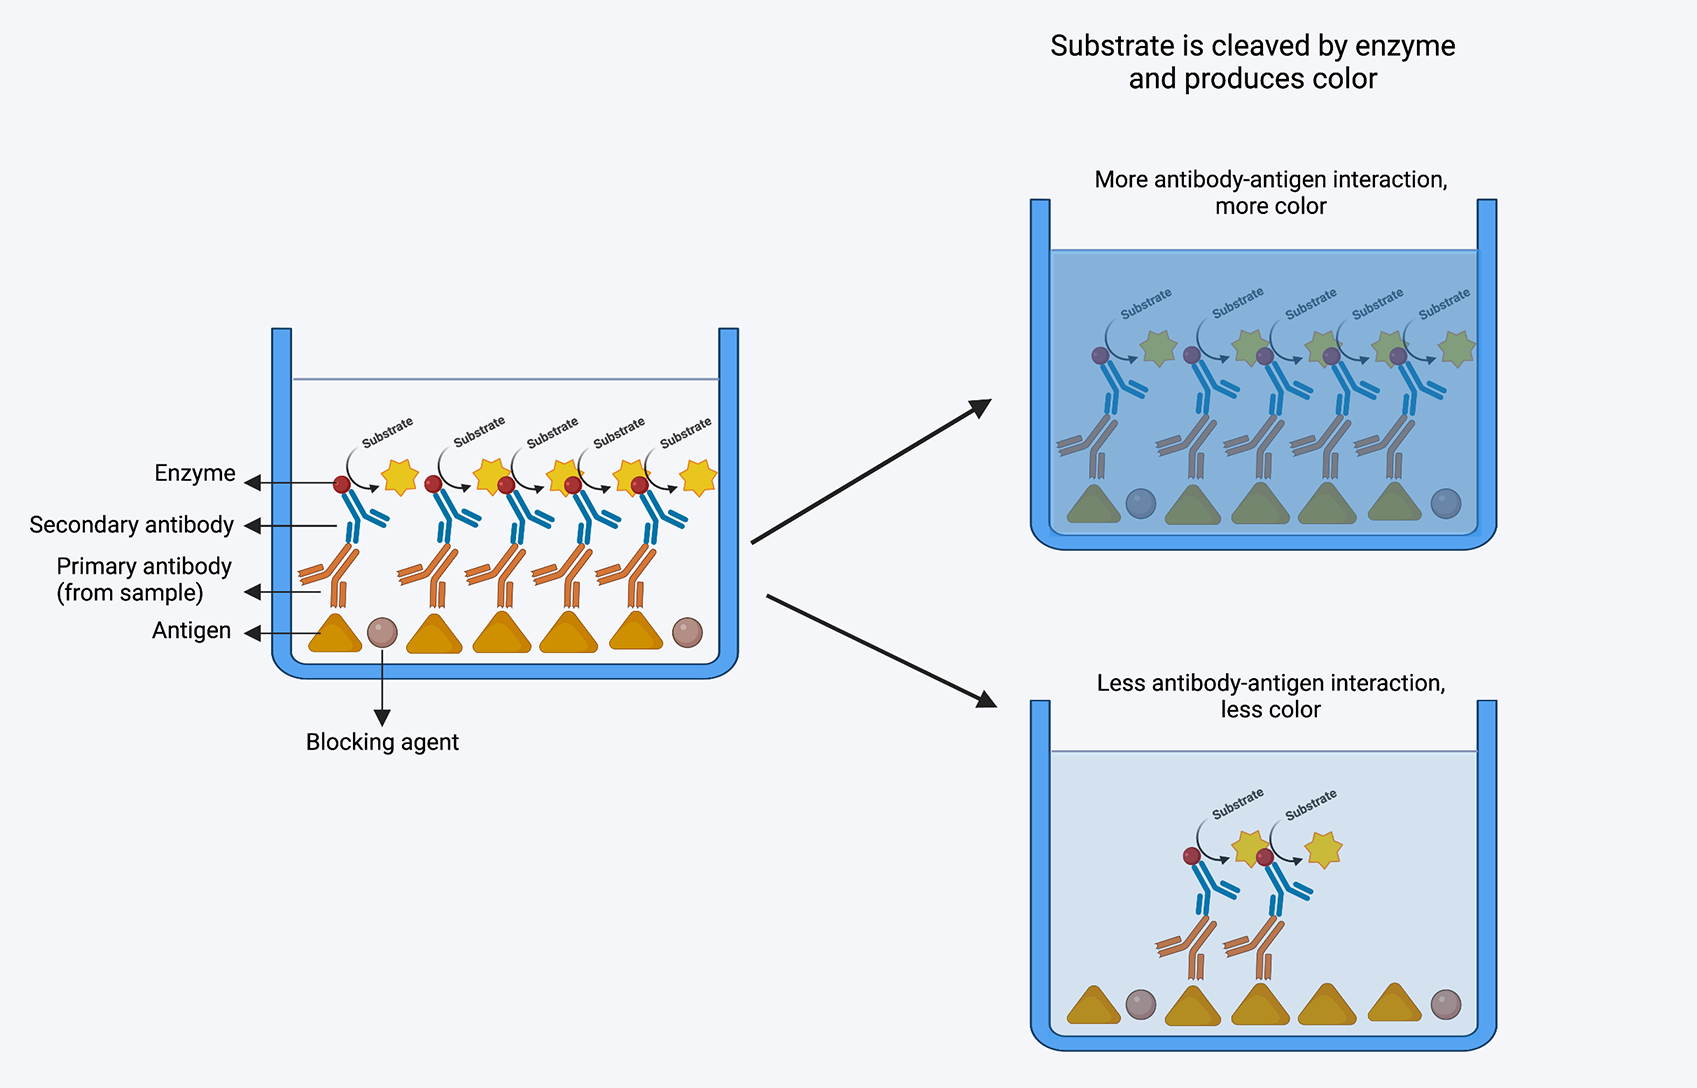
\includegraphics[width=1\linewidth]{DATA/elisa} \caption{A caption}\label{fig:pressure}
\end{figure}

\hypertarget{read-in-data-from-excel-file}{%
\section{Read in data from excel file}\label{read-in-data-from-excel-file}}

\begin{Shaded}
\begin{Highlighting}[]
\NormalTok{elisa\_raw\_data }\OtherTok{\textless{}{-}} \FunctionTok{read\_excel}\NormalTok{(}\StringTok{"DATA/elisa\_s1\_07{-}25{-}20.xlsx"}\NormalTok{, }\AttributeTok{sheet =} \StringTok{"S1"}\NormalTok{, }\AttributeTok{col\_names =} \ConstantTok{FALSE}\NormalTok{,  }\AttributeTok{range =} \StringTok{"B2:M9"}\NormalTok{)}
\end{Highlighting}
\end{Shaded}

\begin{verbatim}
## New names:
## * `` -> ...1
## * `` -> ...2
## * `` -> ...3
## * `` -> ...4
## * `` -> ...5
## * ...
\end{verbatim}

\begin{Shaded}
\begin{Highlighting}[]
\FunctionTok{head}\NormalTok{(elisa\_raw\_data)}
\end{Highlighting}
\end{Shaded}

\begin{verbatim}
## # A tibble: 6 x 12
##   ...1     ...2  ...3 ...4     ...5  ...6 ...7     ...8  ...9 ...10  ...11 ...12
##   <chr>   <dbl> <dbl> <chr>   <dbl> <dbl> <chr>   <dbl> <dbl> <chr>  <dbl> <dbl>
## 1 5.1999~ 0.05  0.069 6.3E-2  0.061 0.122 0.1680~ 0.145 0.135 6.800~ 0.053 0.05 
## 2 7.9000~ 0.098 0.069 6.8000~ 0.115 0.202 5.8999~ 0.134 0.069 0.106  0.05  0.075
## 3 8.8999~ 0.133 0.119 OVRFLW  3.87  2.32  OVRFLW  3.85  2.12  OVRFLW 3.21  1.02 
## 4 OVRFLW  3.46  1.16  OVRFLW  3.80  2.36  OVRFLW  3.70  1.49  OVRFLW 3.68  1.63 
## 5 3.8159~ 1.82  0.446 3.8940~ 3.42  1.13  OVRFLW  2.33  0.608 OVRFLW 3.41  1.10 
## 6 OVRFLW  3.69  1.43  OVRFLW  3.66  1.27  3.839   1.74  0.444 2.499~ 0.637 0.704
\end{verbatim}

\hypertarget{tidy-the-data}{%
\section{Tidy the data}\label{tidy-the-data}}

\begin{Shaded}
\begin{Highlighting}[]
\CommentTok{\# Convert all columns to numeric}

\NormalTok{elisa\_raw\_data\_numeric }\OtherTok{\textless{}{-}}\NormalTok{ elisa\_raw\_data }\SpecialCharTok{\%\textgreater{}\%} 
  \FunctionTok{mutate\_if}\NormalTok{(is.character, as.numeric)}
\end{Highlighting}
\end{Shaded}

\begin{verbatim}
## Warning in mask$eval_all_mutate(quo): NAs introduced by coercion

## Warning in mask$eval_all_mutate(quo): NAs introduced by coercion

## Warning in mask$eval_all_mutate(quo): NAs introduced by coercion

## Warning in mask$eval_all_mutate(quo): NAs introduced by coercion
\end{verbatim}

\begin{Shaded}
\begin{Highlighting}[]
\CommentTok{\# pivot longer the data}

\NormalTok{elisa\_raw\_data\_tidy }\OtherTok{\textless{}{-}} \FunctionTok{pivot\_longer}\NormalTok{(}\AttributeTok{data =}\NormalTok{ elisa\_raw\_data\_numeric, }\AttributeTok{cols =} \StringTok{"...1"}\SpecialCharTok{:}\StringTok{"...12"}\NormalTok{, }\AttributeTok{names\_to =} \StringTok{"well\_id"}\NormalTok{, }\AttributeTok{values\_to =} \StringTok{"od\_450nm"}\NormalTok{)}

\CommentTok{\# remove "..." from the first column}

\NormalTok{elisa\_raw\_data\_tidy}\SpecialCharTok{$}\NormalTok{well\_id }\OtherTok{\textless{}{-}} \FunctionTok{str\_replace}\NormalTok{(elisa\_raw\_data\_tidy}\SpecialCharTok{$}\NormalTok{well\_id, }\StringTok{"..."}\NormalTok{, }\StringTok{""}\NormalTok{)}

\CommentTok{\# Add new column to the data\_frame}

\NormalTok{elisa\_raw\_data\_tidy\_new }\OtherTok{\textless{}{-}}\NormalTok{ elisa\_raw\_data\_tidy }\SpecialCharTok{\%\textgreater{}\%}
  \FunctionTok{mutate}\NormalTok{(}\AttributeTok{name =} \FunctionTok{rep}\NormalTok{(LETTERS[}\DecValTok{1}\SpecialCharTok{:}\DecValTok{8}\NormalTok{], }\AttributeTok{each =} \DecValTok{12}\NormalTok{))}

\NormalTok{elisa\_raw\_data\_tidy\_new }\OtherTok{\textless{}{-}}\NormalTok{ elisa\_raw\_data\_tidy\_new }\SpecialCharTok{\%\textgreater{}\%}
  \FunctionTok{mutate}\NormalTok{(}\AttributeTok{well\_id =} \FunctionTok{paste0}\NormalTok{(name, well\_id)) }\SpecialCharTok{\%\textgreater{}\%}
  \FunctionTok{select}\NormalTok{(}\SpecialCharTok{{-}}\NormalTok{name)}

\FunctionTok{head}\NormalTok{(elisa\_raw\_data\_tidy\_new)}
\end{Highlighting}
\end{Shaded}

\begin{verbatim}
## # A tibble: 6 x 2
##   well_id od_450nm
##   <chr>      <dbl>
## 1 A1         0.052
## 2 A2         0.05 
## 3 A3         0.069
## 4 A4         0.063
## 5 A5         0.061
## 6 A6         0.122
\end{verbatim}

\hypertarget{read-in-second-data-set}{%
\section{Read in second data set}\label{read-in-second-data-set}}

\begin{Shaded}
\begin{Highlighting}[]
\NormalTok{elisa\_label\_data }\OtherTok{\textless{}{-}} \FunctionTok{read\_excel}\NormalTok{(}\StringTok{"DATA/elisa\_s1\_07{-}25{-}20.xlsx"}\NormalTok{, }\AttributeTok{sheet =} \StringTok{"S1"}\NormalTok{, }\AttributeTok{col\_names =} \ConstantTok{FALSE}\NormalTok{,  }\AttributeTok{range =} \StringTok{"Q2:AB9"}\NormalTok{)}
\end{Highlighting}
\end{Shaded}

\begin{verbatim}
## New names:
## * `` -> ...1
## * `` -> ...2
## * `` -> ...3
## * `` -> ...4
## * `` -> ...5
## * ...
\end{verbatim}

\begin{Shaded}
\begin{Highlighting}[]
\FunctionTok{head}\NormalTok{(elisa\_label\_data)}
\end{Highlighting}
\end{Shaded}

\begin{verbatim}
## # A tibble: 6 x 12
##   ...1        ...2   ...3  ...4  ...5  ...6  ...7  ...8  ...9  ...10 ...11 ...12
##   <chr>       <chr>  <chr> <chr> <chr> <chr> <chr> <chr> <chr> <chr> <chr> <chr>
## 1 blank       secon~ naïv~ 1A-1~ 1A-1~ 1A-1~ 1A-2~ 1A-2~ 1A-2~ 1A-3~ 1A-3~ 1A-3~
## 2 1A-4 (1/250 1A-4 ~ 1A-4~ 1B-1~ 1B-1~ 1B-1~ 1B-2~ 1B-2~ 1B-2~ 1B-3~ 1B-3~ 1B-3~
## 3 1B-4 (1/250 1B-4 ~ 1B-4~ 2A-1~ 2A-1~ 2A-1~ 2A-2~ 2A-2~ 2A-2~ 2A-3~ 2A-3~ 2A-3~
## 4 2B-1 (1/250 2B-1 ~ 2B-1~ 2B-2~ 2B-2~ 2B-2~ 2B-3~ 2B-3~ 2B-3~ 2B-4~ 2B-4~ 2B-4~
## 5 3A-1 (1/250 3A-1 ~ 3A-1~ 3A-2~ 3A-2~ 3A-2~ 3A-3~ 3A-3~ 3A-3~ 3A-4~ 3A-4~ 3A-4~
## 6 3B-1 (1/250 3B-1 ~ 3B-1~ 3B-2~ 3B-2~ 3B-2~ 3B-3~ 3B-3~ 3B-3~ 3B-4~ 3B-4~ 3B-4~
\end{verbatim}

\begin{Shaded}
\begin{Highlighting}[]
\CommentTok{\# pivot longer the data}

\NormalTok{elisa\_label\_data\_tidy }\OtherTok{\textless{}{-}} \FunctionTok{pivot\_longer}\NormalTok{(}\AttributeTok{data =}\NormalTok{ elisa\_label\_data, }\AttributeTok{cols =} \StringTok{"...1"}\SpecialCharTok{:}\StringTok{"...12"}\NormalTok{, }\AttributeTok{names\_to =} \StringTok{"well\_id"}\NormalTok{, }\AttributeTok{values\_to =} \StringTok{"information"}\NormalTok{)}

\CommentTok{\# remove "..." from the first column}

\NormalTok{elisa\_label\_data\_tidy}\SpecialCharTok{$}\NormalTok{well\_id }\OtherTok{\textless{}{-}} \FunctionTok{str\_replace}\NormalTok{(elisa\_label\_data\_tidy}\SpecialCharTok{$}\NormalTok{well\_id, }\StringTok{"..."}\NormalTok{, }\StringTok{""}\NormalTok{)}

\CommentTok{\# Add new column to the data\_frame}

\NormalTok{elisa\_label\_data\_tidy\_new }\OtherTok{\textless{}{-}}\NormalTok{ elisa\_label\_data\_tidy }\SpecialCharTok{\%\textgreater{}\%}
  \FunctionTok{mutate}\NormalTok{(}\AttributeTok{name =} \FunctionTok{rep}\NormalTok{(LETTERS[}\DecValTok{1}\SpecialCharTok{:}\DecValTok{8}\NormalTok{], }\AttributeTok{each =} \DecValTok{12}\NormalTok{))}

\NormalTok{elisa\_label\_data\_tidy\_new }\OtherTok{\textless{}{-}}\NormalTok{ elisa\_label\_data\_tidy\_new }\SpecialCharTok{\%\textgreater{}\%}
  \FunctionTok{mutate}\NormalTok{(}\AttributeTok{well\_id =} \FunctionTok{paste0}\NormalTok{(name, well\_id)) }\SpecialCharTok{\%\textgreater{}\%}
  \FunctionTok{select}\NormalTok{(}\SpecialCharTok{{-}}\NormalTok{name)}

\FunctionTok{head}\NormalTok{(elisa\_label\_data\_tidy\_new)}
\end{Highlighting}
\end{Shaded}

\begin{verbatim}
## # A tibble: 6 x 2
##   well_id information  
##   <chr>   <chr>        
## 1 A1      blank        
## 2 A2      secondary    
## 3 A3      naïve (1/250)
## 4 A4      1A-1 (1/250  
## 5 A5      1A-1 (1/1250 
## 6 A6      1A-1 (1/6250
\end{verbatim}

\hypertarget{join-the-od-table-with-the-information-table}{%
\section{Join the OD table with the information table}\label{join-the-od-table-with-the-information-table}}

\begin{Shaded}
\begin{Highlighting}[]
\NormalTok{elisa\_data }\OtherTok{=}\NormalTok{ elisa\_raw\_data\_tidy\_new }\SpecialCharTok{\%\textgreater{}\%} \FunctionTok{inner\_join}\NormalTok{(elisa\_label\_data\_tidy\_new, }\AttributeTok{by=}\StringTok{"well\_id"}\NormalTok{)}

\FunctionTok{head}\NormalTok{(elisa\_data)}
\end{Highlighting}
\end{Shaded}

\begin{verbatim}
## # A tibble: 6 x 3
##   well_id od_450nm information  
##   <chr>      <dbl> <chr>        
## 1 A1         0.052 blank        
## 2 A2         0.05  secondary    
## 3 A3         0.069 naïve (1/250)
## 4 A4         0.063 1A-1 (1/250  
## 5 A5         0.061 1A-1 (1/1250 
## 6 A6         0.122 1A-1 (1/6250
\end{verbatim}

\hypertarget{separate-the-information-tabke-into-sample-id-and-dilution-columns}{%
\section{Separate the information tabke into sample ID and dilution columns}\label{separate-the-information-tabke-into-sample-id-and-dilution-columns}}

\begin{Shaded}
\begin{Highlighting}[]
\NormalTok{tidy\_elisa\_data }\OtherTok{\textless{}{-}} \FunctionTok{separate}\NormalTok{(elisa\_data, }\AttributeTok{col =} \StringTok{"information"}\NormalTok{, }\AttributeTok{into =} \FunctionTok{c}\NormalTok{(}\StringTok{"sample\_id"}\NormalTok{, }\StringTok{"dilution"}\NormalTok{), }\AttributeTok{sep =} \StringTok{"}\SpecialCharTok{\textbackslash{}\textbackslash{}}\StringTok{("}\NormalTok{)}
\end{Highlighting}
\end{Shaded}

\begin{verbatim}
## Warning: Expected 2 pieces. Missing pieces filled with `NA` in 2 rows [1, 2].
\end{verbatim}

\begin{Shaded}
\begin{Highlighting}[]
\FunctionTok{head}\NormalTok{(tidy\_elisa\_data)}
\end{Highlighting}
\end{Shaded}

\begin{verbatim}
## # A tibble: 6 x 4
##   well_id od_450nm sample_id   dilution
##   <chr>      <dbl> <chr>       <chr>   
## 1 A1         0.052 "blank"     <NA>    
## 2 A2         0.05  "secondary" <NA>    
## 3 A3         0.069 "naïve "    1/250)  
## 4 A4         0.063 "1A-1 "     1/250   
## 5 A5         0.061 "1A-1 "     1/1250  
## 6 A6         0.122 "1A-1 "     1/6250
\end{verbatim}

\begin{Shaded}
\begin{Highlighting}[]
\NormalTok{tidy\_elisa\_data }\OtherTok{\textless{}{-}}\NormalTok{ tidy\_elisa\_data }\SpecialCharTok{\%\textgreater{}\%}
  \FunctionTok{mutate}\NormalTok{(}\AttributeTok{dilution =} \FunctionTok{str\_extract}\NormalTok{(dilution, }\StringTok{"(/)[0{-}9]+"}\NormalTok{),}
         \AttributeTok{dilution =} \FunctionTok{str\_replace}\NormalTok{(dilution, }\StringTok{"/"}\NormalTok{, }\StringTok{""}\NormalTok{),}
         \AttributeTok{dilution =} \FunctionTok{as.numeric}\NormalTok{(dilution))}

\NormalTok{tidy\_elisa\_data }\OtherTok{\textless{}{-}}\NormalTok{ tidy\_elisa\_data }\SpecialCharTok{\%\textgreater{}\%}
  \FunctionTok{select}\NormalTok{(well\_id, sample\_id, dilution, od\_450nm)}

\FunctionTok{head}\NormalTok{(tidy\_elisa\_data)}
\end{Highlighting}
\end{Shaded}

\begin{verbatim}
## # A tibble: 6 x 4
##   well_id sample_id   dilution od_450nm
##   <chr>   <chr>          <dbl>    <dbl>
## 1 A1      "blank"           NA    0.052
## 2 A2      "secondary"       NA    0.05 
## 3 A3      "naïve "         250    0.069
## 4 A4      "1A-1 "          250    0.063
## 5 A5      "1A-1 "         1250    0.061
## 6 A6      "1A-1 "         6250    0.122
\end{verbatim}

\hypertarget{elisa-data-analysis-optimization}{%
\section{ELISA data analysis optimization}\label{elisa-data-analysis-optimization}}

  \bibliography{book.bib,packages.bib}

\end{document}
